\documentclass[letterpaper, 10 pt, conference]{ieeeconf} % letterpaper/a4paper 
% ieeeconf IEEEtran
\IEEEoverridecommandlockouts   % Needed if you want to use the \thanks command
\overrideIEEEmargins

\usepackage[ruled,vlined]{algorithm2e}
\usepackage{amsmath}
\usepackage{amsfonts}
\usepackage{graphicx}
\usepackage{verbatim}

\DeclareMathOperator*{\argmin}{arg\,min}
\DeclareMathOperator*{\argmax}{arg\,max}
\newcommand{\vect}[1]{\mathbf{#1}}
\newcommand{\hvect}[1]{\bar{\vect{#1}}}
\newcommand{\uvect}[1]{\hat{\vect{#1}}}
\newcommand{\field}[1]{\mathbb{#1}}
\newcommand{\Real}[0]{\field{R}}


\title{Modern MAP methods for accurate and faster occupancy grid mapping}
\author{Vikas Dhiman, Brian, Jason J. Corso, Abhijit Kundu, Frank Dallert}
\begin{document}
\maketitle
\begin{abstract}
  Most occupancy grid mapping algorithms have been using two assumption
  algorithm.  \cite{merali2013icra} showed that belief maximization methods
  produce better maps than the traditional two assumption algorithm.  In this
  paper, we show that we can go beyond methods like MCMC Gibbs sampling and
  obtain faster convergence by using modern methods like Sum Product algorithm
  and Dual Decomposition.
\end{abstract}
\section{Introduction}
% navigation -> localization and mapping -> mapping
%Autonomous navigation of mobile robots is an important problem for any kind of robot that needs to find s path through obstacles.
Robotic mapping is an important problem. It is a necessary step for applications like indoor autonomous navigation, grasping, reconstruction and augmented reality. It is often done in parallel with localization and termed as Simultaneous localization and mapping. Given the importance of the problem, lot of work has been done in this field. The approaches discussed in literature have used various kinds of sensors 
Sonars,%TODO: cite sonar mapping papers,
laser scanners, %TODO : cite laser mapping papers
simple cameras, %TODO : single camera reconstructions
RGB-D Cameras \cite{newcombe2011kinectfusion, whelan2013robust, whelan2012kintinuous}. 
However, all the mapping algorithms introduced in the robotics suffer use a inaccurate independent cell assumption as pointed out in the % TODO: cite thrun's paper

The main reason for using this assumption is speed gain that we gain with the independent cell assumption. We show that the assumption if dropped can produce more accurate maps, which can be useful when more accurate reconstructions are required and when computational resources are not limited, for example, during post processing of the data.

We introduce the factor graph approach of solving mapping problem which, to the best of our knowledge, has not been introduced to the robotics community. The closest work is that of \cite{merali2013icra} that uses Monte carlo Markov chain (MCMC) methods to estimate accurate maps. It has been a common knowledge that MCMC methods are very likely to get stuck in a local minimum. In this paper, we go beyond MCMC methods and evaluate modern factor graph optimization methods to compute maps that are more accurate given the accuracy as long as we have an accurate forward sensor model.


\section{Related work}
% Work that has been in "application" i.e. mapping

% Itersection mapping using forward sensor models
% Thrun03ar:
% Standard occupancy methods are characterized by two algorith-
% mic choices:
% 1. They decompose the high-dimensional mapping problem into many binary estimation
% problems, which are then solved independently of each other.
% 2. They rely on inverse models of the robot’s sensors which reasons from sensor measure-
% ments to maps (opposite of the way sensor data is generated).
\cite{thrun2003learning} made an argument for using forward sensor models in sonar based mapping instead of conventional inverse sensor model.


% Work that has been in done in "method" that i.e MAP
Minimization of cost (or energy) function over Factor graphs is a well studied field and it has found numerous application in the field of information theory, computer vision and machine learning. A lot of work has been done in the field.

\section{Problem definition}
\newcommand{\map}{\vect{x}}
A robot equipped with a laser scanner and accurate odometry moves in a static
environment, problem is to figure out an optimal occupancy grid map. For the
purpose of ground robots often 2D maps are enough for path planning and
exploration.
% define problem in probability terms
The area to be mapped is divided into $N$ discrete cells. Let $x_i$ denote the state of cell $i$, which can take values from label set $L_i = \{0, 1\}$, where $0$ (resp. $1$) denotes that cell is free (resp. occupied). We define, the map $\map$ as a vector that defines state for all $N$ cells, $\map = [x_i]^\top_{1 \le i \le N}$. Hence map $\map$ takes values from sample space $\Omega = \prod_{1 \le i \le N}L_i$.

Let $z_t$ denote the $t$\textsuperscript{th} laser range measurement when captured from pose $\rho_t$. We assume that the probability of observation $p(z_t| \rho_t, \map)$ (forward sensor model) be given. The problem is to find the probability of all cells $i$ being occupied given all observations $z = [z_f]^\top_{1 \le f \le t}$ and $\rho = [\rho_f]^\top_{1 \le f \le t}$.
\begin{align}
  p(x_i = 1 | z, \rho) &= \sum_{\map \in \Omega : x_i = 1} p(\map | z , \rho) & \forall 1 \le i \le N 
  \label{eq:fullsolution}
\end{align}
In another formulation of problem, we can focus on the best overall occupancy of the map that maximizes the posterior probability:
\begin{align}
  \vect{x}* &= \argmax_{\map \in \Omega } p(\map | z, \rho)
  \label{eq:mapproblem}
\end{align}
It is easy to see that any solution to this problem would have complexity that is exponential in the number of cells. We can only hope to find an approximate solution of this problem.

\section{Mapping by inverse sensor model}
% assume independence
%\eqref{eq:fullsolution} is usually simplified in robotic mapping algorithms by introducing two assumptions:
Commonly used occupancy grid mapping algorithms make simplifying assumption
that each grid cell is independent of all other map cells. 
%As a result instead of the static world assumption (\eqref{eq:staticWorldAssumption}), we use 
\begin{align}
  %p(z_t|x_i, \sigma_{1:t-1}, \rho_t) = p(z_t|x_i, \rho_t)
  p(x_i|z, \rho) &= \frac{p(z_t, \rho_t|x_i, \sigma_{1:t-1})p(x_i|\sigma_{1:t-1})}
                         {p(z_t, \rho_t|\sigma_{1:t-1})}
\end{align}
% Thrun03ar : A common assumption in mapping is the static world assumption, which states that past sensor readings are conditionally independent given knowledge of the map \map, for any point in time t:
The current laser measurement $z_t$ are commonly assumed (static world assumption) \cite{thrun2003learning} to be independent of previous observations $\sigma_{1:t-1}$ given the map $x_i$ :
\begin{align}
  p(z_t, \rho_t|x_i, \sigma_{1:t-1}) &= p(z_t, \rho_t|x_i)
 \label{eq:staticWorldAssumption}
\end{align}
Using static world assumption (\eqref{eq:staticWorldAssumption}), we get:
\begin{align}
 p(x_i|z, \rho) &= p(z_t, \rho_t|x_i)\frac{p(x_i|\sigma_{1:t-1})}
                                           {p(z_t, \rho_t|\sigma_{1:t-1})}\\
                 &= \frac{p(x_i|z_t, \rho_t)p(z_t,\rho_t)} {p(x_i)}\frac{p(x_i|\sigma_{1:t-1})}{p(z_t, \rho_t|\sigma_{1:t-1})}\\
                 &= \frac{1}{Z'}\frac{p(x_i|z_t, \rho_t)p(x_i|\sigma_{1:t-1})}{p(x_i)}\\
                 &= \frac{1}{Z'}\prod_{1\le f \le t} \frac{p(x_i|z_f, \rho_f)}{p(x_i)}
\end{align}
where $Z'$ is a normalizing factor that is independent of $x_i$.


\section{Mapping by forward sensor model}

   Here we present minimum assumption simplification of
   \eqref{eq:fullsolution} as done in \cite{thrun2003learning,
   merali2013icra}. 
   For conciseness, we use 
   %$\sigma_t = \{z_t, \rho_t\}$ to represent both range and pose of $t$\textsuperscript{th} laser measurement.
   %Similarly,
   $\sigma_{1:t-1} = \{z_{1:t-1}, \rho_{1:t-1}\}$ to represent all but
   $t$\textsuperscript{th} measurement. For a given map $\map$, the conditional
   probability of map being correct is
   \begin{align}
     p(\map | z, \rho) &= p(\map | \sigma_{1:t-1}, z_t, \rho_t)\\
                    &= \frac{p(z_t|\map , \sigma_{1:t-1}, \rho_t)p(\map| \sigma_{1:t-1}, \rho_t)}
                            {p(z_t|\sigma_{1:t-1}, \rho_t)}
     \label{eq:recursivesol}
   \end{align}
   Static world assumption, $p(z_t|\map, \sigma_{1:t-1}, \rho_t) = p(z_t|\map, \rho_t)$, simplifies \eqref{eq:recursivesol} to :
   \begin{align}
     p(\map|z, \rho) &= \frac{p(z_t|\map, \rho_t)p(\map| \sigma_{1:t-1}, \rho_t)}
                          {p(z_t|\sigma_{1:t-1}, \rho_t)}\\
                  &= \frac{p(z_t|\map, \rho_t)p(\rho_t|\map, \sigma_{1:t-1})p(\map| \sigma_{1:t-1})}
                          {p(z_t|\sigma_{1:t-1}, \rho_t)p(\rho_t|\sigma_{1:t-1})}
   \end{align}

   Another common assumption is that the pose of robot $\rho_t$ being independent of map $\map$:
   \begin{align}
     p(\rho_t|\map, \sigma_{1:t-1}) = p(\rho_t|\sigma_{1:t-1})
   \end{align}
   Using independent pose assumption, we get a recursive formula for \eqref{eq:recursivesol}
   \begin{align}
     p(\map | z, \rho) &= \frac{1}{Z} p(z_t|\map , \rho_t)p(\map| z_{1:t-1}, \rho_{1:t-1})\\
                       &= \frac{1}{Z} \prod_{1 \le f \le t} p(z_f|\map, \rho_f)
     \label{eq:map}
   \end{align}
   where $Z$ is a normalizing constant independent of $\map$. The term $p(z_f|\vect{x}, p_f)$ is the \emph{forward sensor model}. Thrun et al. \cite{thrun2003learning} approach this problem by expectation maximization, while Merali et al. \cite{merali2013icra} use Gibbs sampling to find approximate solution. In this paper, we explore modern explore modern methods of finding maximum a posteriori estimate of this problem.

   Modern MAP methods approach the problem \eqref{eq:map}, by making use of the fact that a laser measurement depends only a small portion of the entire map:
   \begin{align}
     p(z_f |\vect{x}, \rho_f) = p(z_f|\vect{x}_f, \rho_f)
   \end{align}
   where $\vect{x}_f \subseteq \vect{x}$ is the small portion of the map on which the laser measurement $f$ depends. Rewriting, \eqref{eq:map} in new notation:
   \begin{align}
     p(\map | z, \rho) &= \frac{1}{Z} \prod_{1 \le f \le t} p(z_f|\map_f, \rho_f)
     \label{eq:modernmap}
   \end{align}
   %However, the full solution is computationally intractable as its complexity is exponential in the number of cells.
%\end{comment}


\section{Representation as factor graph and Notation}
\label{sec:notation}
The problem of Occupancy grid mapping can be expressed as energy minimization
over a factor graph. Let all cells in the map be the variable nodes $V$ and all
the laser measurements be factor nodes $F$. 
There exists an undirected edge $(i, f)$, if and only if the laser
range measurement $p(z_f|\vect{x}, \rho_f)$ depends on the cell occupancy 
$x_i$. In this paper, we assume that laser range measurement depends on only
those cells that the laser passes through for given pose $\rho_f$. Though more
complicated models can lead to better accuracy, we show that with such a simple
model we are able to achieve better accuracy than methods tried so far.
Let $E$ be set of all such edges:
% Mathematically,
\begin{align}
  E = \{(i, f) : i \in V, f \in F, \text{laser $f$ passes through cell $i$}\}
\end{align}
This defines our factor graph representation of occupancy grid mapping $G = (V, F, E)$.

%Let $n(.)$ denote neighborhood in factor graph $G = \{V, F, E\}$.
%
%% unncessary
% i.e
% \begin{align}
%   n(k) &= \begin{cases}
%   \{f \in F: (i, f) \in E\} & \text{ if $k \in V$}\\
%   \{i \in V: (i, f) \in E\} & \text{ if $k \in F$}
%   \end{cases}
% \end{align}
%
% As before each cell $i \in V$ takes values
% from a discrete set of labels $L_i = \{0, 1\}$, where $0$ (respectively $1$) means that
% the cell is free (respectively occupied). Also denote the sample space of all the
% cells in the map as $\Omega = \prod_{i \in V} L_i$.

% Each laser measurement $f \in F$ corresponds to a function $\theta_f : \vect{x}_f \rightarrow \Real$ 
% that depends only on the labels of the neighboring cells, $\vect{x}_f = \{x_i\}_{i
% \in n(f)}$, and evaluates to an
% \emph{energy} value. Here $n(.)$ denotes the neighborhood in the factor graph $G$.
% The \emph{energy} can be thought as the negative log likelihood of the given
% state $\vect{x}_f$ being the correct state according to the laser measurement $f$.

% In this formulation, we seek to determine the label of all the map cells that
% maximizes the total likelihood across all measurements, which is equivalent to
% minimizing the total \emph{energy} over all factors.
We focus on the maximum-a-posteriori formulation of the problem (using equations \eqref{eq:mapproblem} and \eqref{eq:modernmap}) 
\begin{align}
  \vect{x}* = \argmax_{\vect{x} \in \Omega} \frac{1}{Z} \prod_{f \in F} p(z_f|\map_f, \rho_f)
  \label{eq:probablisticmap}
\end{align}
Often, for computational reasons, this problem is approached in negative log
likelihood or \emph{energy} domain. Let 
$\theta_f(\vect{x}_f) = - \log p(z_f|\map_f, \rho_f)$ 
denote the \emph{energy} for the laser measurement $f$. Note that here we
assume that $p(z_f|\map_f, \rho_f) > 0$, which is practically achievable by
choosing very low probability values instead of zero for highly improbable
cases.  Taking negative log on both sides of \eqref{eq:probablisticmap} and
dropping the constant normalizing factor, we get:
\begin{align}
  \vect{x}* = \argmin_{\vect{x} \in \Omega} \sum_{f \in F} \theta_f(\vect{x}_f)
\end{align}
\begin{figure}
  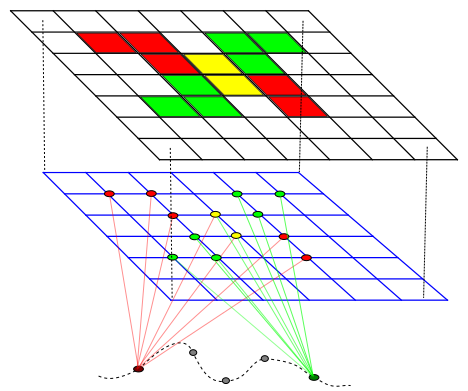
\includegraphics[width=\columnwidth]{../figures/factorgraph/factorgraph.pdf}
  \caption{Diagrammatic conversion of Occupancy Grid to a factor graph.}
  \label{fig:factor-graph}
\end{figure}

\section{Forward sensor models}
We explore here a few plausible sensor models
\subsection{Gaussian sensor model}
\newcommand{\actz}{\bar{z}_f(\vect{x}_f, \rho_f)}
In this sensor model, we assume that the laser measurements are affected by Gaussian noise. The forward sensor model is given by
\begin{align}
  p(z_f|\vect{x}_f, \rho_f) &= \frac{1}{2\pi\sigma}\exp\left(-\frac{(\actz - z_f)^2}{\sigma^2}\right)
\end{align}
where $\actz$ is the distance of first occupied cell in $\vect{x}_f$ starting from pose $\rho_f$. Also $\sigma$ is a measure of noise in laser measurement and it often depends on the distance measured. For our experiments we assume noise to linearly vary with distance as $\sigma = \sigma_0z_f$. 

In terms of negative log likelihood, the energy function becomes
\begin{align}
  \theta_f(\vect{x}_f) &= \frac{1}{\sigma_0^2}\left(1 - \frac{\actz}{z_f}\right)^2 + \log(2\pi\sigma_0z_f)
\end{align}
% In terms of discrete set of cells that the laser passes through the energy function becomes
% \begin{align}
%   \theta_f(\vect{x}_f) &= \frac{1}{\sigma_0^2}\left(1 - \frac{\kappa(\vect{x}_f) \Delta}{z_f}\right)^2 + \log(2\pi\sigma_0z_f)
% \end{align}
% where $\kappa(\vect{x}_f)$ denote the index of the first occupied cell in $\vect{x}_f$ and $\Delta$ is the cell size.

\subsection{Piecewise constant sensor model}
The expected pattern of occupancy from a laser observation is two have last cell as occupied and others as free. So the simplest energy function would be 
\begin{align}
  \theta_f(\vect{x}_f) &= \begin{cases}
              0 & \text{ if } \vect{x}_f = [0, 0 \dots 0, 1]^\top\\
           1000 & \text{ otherwise}
  \end{cases}
\end{align}
where $[0, 0 \dots 0, 1]$ means that all cells are $0$ except the last cell which is $1$. In this context, we consider $\vect{x}^f$ to be a vector of ordered cell labels through which laser measurement $f$ passes.

However, to resolve conflicts it is sometimes better to provide lower energy to all cells free case. Hence, we come with the following energy function.
\begin{align}
  \theta_f(\vect{x}_f) &= \begin{cases}
                     0 & \text{ if } \vect{x}_f = \vect{P}_1\\
                   900 & \text{ if } \vect{x}_f = \vect{P}_2\\
                  1000 & \text{ otherwise}
  \end{cases}
\end{align}
where $\vect{P}_1 = [0, 0 \dots 0, 1]^\top$ and $\vect{P}_2 = [0, 0 \dots 0, 0]^\top$.
\section{Metropolis hastings}
Markov Chain Monte Carlo (MCMC) methods allow us to sample from high dimensional probability distributions. The samples drawn using MCMC methods are not independent but correlated as a Markov chain. They work by moving in a random walk in the high dimensional space. Metropolis Hastings is one of the popular MCMC methods. The idea is to sample $\vect{x}$ from the probability distribution $p(\vect{x}|z, \rho)$ and after sufficient number of iterations, we should get sample that is close to the true map.

In general, for Metropolis hastings a \emph{transition probability} $Q(\vect{x}',
\vect{x}^r)$ is chosen, that depends on current sample $\vect{x}^r$ and guides the random
walk in the high-dimensional space. We randomly sample a point $\vect{x}'$ 
from from $Q(.)$ and it is either accepted or rejected based on the acceptance probability $a$:
\begin{align}
  a = \frac{p(\vect{x}'|z, \rho)Q(\vect{x}^r, \vect{x}')}
  {p(\vect{x}^r|z, \rho)Q(\vect{x}', \vect{x}^r)}
\end{align}
\begin{align}
  \vect{x}^{r+1} = \begin{cases}
    \vect{x}' & \text{ if $a \ge 1$ or with Probability $a$  }\\
    \vect{x}^r & \text{ otherwise}\\
  \end{cases}
\end{align}
Interested reader is referred to \cite{mackay1998introduction}.
\subsection{Heat map}
\section{Sum product}
\cite{kschischang2001factor} introduced the algorithm.
\subsection{Efficient sum product}
\section{Dual decomposition}
\newcommand{\msg}[3]{\mu_{#1#2}(#3)}
\newcommand{\assign}{\leftarrow}
\newcommand{\Sx}{L_i}
Dual decomposition algorithm employs Lagrangian relaxation technique from integer programming to minimize. Here we explain the implementation of the algorithm without going into mathematical derivations. Interested user is referred to \cite{sontag2011introduction,jojic2010accelerated,komodakis2009beyond} for proofs and more variations of the algorithm. 

Pseudo code for Dual decomposition is provided in Alg~\ref{alg:dualdecompostion}. Apart from input factor graph $G = (V, F, E)$ and label set $\{\Sx\}_{i \in V}$ introduced in Sec~\ref{sec:notation}, Dual decomposition depends on a step size $\alpha$.

The idea for Dual decomposition is to split the minimization problem into \emph{slave} problems that can be efficiently minimized. In case of disagreement for minimizing label among slave problems, the messages to slave problems are updated until the slave problems agree with each other. We maintain the minimizing label for variable node $i$, computed by slave problem corresponding to $f$ as $x^f_i$. Also, we use $\msg{i}{f}{x_i}$ to denote messages from node $i$ to slave problem corresponding to $f$ regarding state $x_i$.

In each iteration of Dual Decomposition, we first minimize all the slave problems getting labels for each pair of variable followed by message update in case of disagreement. Optionally, we can only minimize only those factors that have at least one disagreeing node in their neighborhood.

\begin{algorithm}
  \dontprintsemicolon
  \KwData{\;
  Factor Graph $G = (V, F, E)$\;
  Label set $\{\Sx\}_{i \in V}$\;
  Step size $\alpha > 0$\;
  Maximum number of iterations $N$\;
  }
  \KwResult{Labels $\{x^f_i\}_{(i, f) \in E} $,
  Messages $\{\msg{i}{f}{x_i}\}$}

  $\msg{i}{f}{x_i} \assign 0 \hfill \forall (i, f) \in E, x_i \in \Sx$\;
  $r \assign 1$\;
  \While{$r < N$} {
    \tcp{For disagreeing factors}
    \For {$f \in F$} {% : \exists i, i' \in n(f) : x_i^f \ne x_{i'}^f$} {
      $\vect{x}^f \assign \argmin\limits_{\vect{x}^f} \left( \theta_f(\vect{x}^f) + \sum\limits_{i \in n(f)}\msg{i}{f}{x^f_i} \right)$\;
    }
    \tcp{For disagreeing nodes}
    \For {$i \in V : \exists f, f' \in n(i) : x_i^{f'} \ne x_i^f$} {
      \For{$f \in n(i)$}{
        $\msg{i}{f}{x^f_i} \assign \msg{i}{f}{x^f_i} + \frac{\alpha}{r}$\;
      }
    }
    $r \leftarrow r + 1$\;
  }
  \label{alg:dualdecompostion}
  \caption{Subgradient Dual Decomposition}
\end{algorithm}
We can compute the minimum energy assignment from dual decomposition messages.
\begin{align}
  x_i \assign \argmax\limits_{x_i \in \Sx} \sum\limits_{f \in n(i)} \msg{i}{f}{x_i}
\end{align}
However, the above computation is only valid if the node has at least a pair of disagreeing factors. In case of agreement, we simply take the agreed upon assignment or if the node is not connected to any factors, we take a random assignment.
%%%%%%%%%%%%%%%%%%%%%%%%%%%%%%%% Unncessary
% \begin{algorithm}
%   \dontprintsemicolon
%   \KwData{\;
%     The Variable Node $i \in V$\;
%     Factor Graph $G = (V, F, E)$\;
%     Label set $\Sx$\;
%     Labels $\{x^f_i\}_{f \in n(i)} $\;
%     Messages $\{\msg{i}{f}{x_i}\}$\;
%   }
%   \KwResult{Minimum energy label $x_i$}
%   \tcc{Check for disagreement}
%   \If{$\exists f, f' \in n(i) : x^{f'}_i \ne x^f_i$}{
%     $x_i \assign \argmax\limits_{x_i \in \Sx} \sum\limits_{f \in n(i)} \msg{i}{f}{x_i}$\;
%   } \Else {
%     \tcc{Take any agreed label}
%     $x_i \assign x^f_i : f \in n(i)$\;
%   }
%   \caption{Label from Dual decomposition messages }
%   \label{alg:compute-assignment}
% \end{algorithm}
%%%%%%%%%%%%%%%%%%%%%%%%%%%%%%%% Unncessary
\subsection{Efficient slave minimization of piecewise constant factor}
Minimizing slave problem can be done efficiently for specific kinds of functions, for example, piecewise constant functions.
The problem is to minimize the energy function along with the received messages.
\begin{align}
  \min_{\vect{x}^f} \left( \theta(\vect{x}^f) + \sum_{i \in n(f)}\msg{i}{f}{x^f} \right)
\end{align}
A general minimization algorithm will take time of the order that is exponential in the number of cells a laser passes through as $\vect{x}^f$ can have $|L_i|^{|n(f)|}$ possible values. However, for our sensor model we can make use of the fact that the piecewise function needs to look for only two patterns. We should compute the total function value for these two patterns and the minimum value for the \emph{otherwise} case. 
\begin{align}
    \min \theta_f(\vect{x}_f) = \min &\left( 0 + \sum_{\vect{x}_f = \vect{P}_1, i \in n(f)}\msg{i}{f}{x_i},\right.\\
                            &900 + \sum_{\vect{x}_f = \vect{P}_2, i \in n(f)}\msg{i}{f}{x_i},\\
                            &\left.1000 + \min_{\vect{x}_f \not\in \{\vect{P}_1, \vect{P}_2\}} \sum_{i \in n(f)}\msg{i}{f}{x_i} \right)
\end{align}
The third term can be easily minimized by 
%choosing the minimizing state for each $i$ over all possible $\Omega(\vect{x}_f)$ by 
simply choosing the minimizing $x_i \in L_i$ for each $i$. However, the minimizing labels can coincide with patterns $\vect{P}_1$ and $\vect{P}_2$. The solution is to find minimum three assignments of $\sum_{i \in n(f)}\msg{i}{f}{x_i}$ and pick the one that is not equal to $\vect{P}_1$ nor $\vect{P}_2$. 

%
% Algorithm~\ref{alg:efficient-minimize} gives pseudo code for minimizing the last term.
% \begin{algorithm}
%   \SetKwFunction{ArgSortNElements}{ArgSortNElements}
%   $e_i = \min\limits_{x_i \in L_i} \msg{i}{f}{x_i} \hfill, \forall i \in n(f)$\;
%   $x^*_i = \argmin\limits_{x_i \in L_i} \msg{i}{f}{x_i} \hfill, \forall i \in n(f)$\;
%   $\delta_{if}(x_i) = \msg{i}{f}{x_i} - e_i \hfill, \forall i \in n(f), x_i \in L_i, x_i \ne x^*_i$\;
%   $I = \ArgSortNElements(\delta_{if}(x_i), \lceil{\log_{|L_i|}{3}}\rceil)$\;
%   \caption{Efficient minimization of piecewise constant function}
%   \label{alg:efficient-minimize}
% \end{algorithm}

\subsection{Selection of step size}
Step size is critical choice as it affects the speed with which Dual decomposition converges. Fig~\ref{fig:dualdecomposition-stepsize} shows convergence with different step size.
\begin{figure}
  \includegraphics[width=\columnwidth]{../figures/dualdecomposition-stepsize-inc500.pdf}
  \caption{The rate of convergence in dual decomposition depends on step size}
  \label{fig:dualdecomposition-stepsize}
\end{figure}
\section{Belief propagation with disagreement tracking}
Intuitively, dual decomposition converges faster because it focuses on the disagreeing 

\section{Experiments} 
Used player and stage to generate simulated data. Input map is in Fig
\begin{figure}
  %\includegraphics[width=\columnwidth]{../figures/hospital_trajectory.png}
\end{figure}
Sampling algorithms are liable to getting stuck in a local minima because we flip only one cell at a time.

\begin{figure}
  \includegraphics[width=\columnwidth]{../figures/relativeconvergence.pdf}%
  \caption{Comparison of convergence of different algorithms on occupancy grid graph. While sampling methods like Metropolis hastings converge quickly they stay far from optimum energy. On the other hand modern minimization algorithms reach closer to an optimum value.}
  \label{fig:convergence-comparison}
\end{figure}
\begin{figure*}
  \includegraphics[width=0.2\textwidth]{../figures/cave_trajectory.png}%
  \includegraphics[width=0.2\textwidth]{../figures/gt-final.png}%
  \includegraphics[width=0.2\textwidth]{../figures/bpresults_100x100_200sec.png}%
  \includegraphics[width=0.2\textwidth]{../figures/SICKDDMCMC200sec_100x100.png}\\
  \includegraphics[width=0.2\textwidth]{../figures/SICKSlowMetropolis200sec_100x100.png}%
  \includegraphics[width=0.2\textwidth]{../figures/dualdecomposition200sec_100x100.png}%
  \includegraphics[width=0.2\textwidth]{../figures/TwoAssumptionAlgo200sec_100x100.png}%
  \caption{Qualitative results at the end of 200sec for each algorithm (from left to right) a) Trajectory of th robot b) Ground truth as observed by robot c) Belief Propagation d) Metropolis Hastings with heat map e) Metropolis Hastings without heat map f) Dual decomposition g) Two assumption algorithm}
  \label{fig:convergence-comparison-visuals}
\end{figure*}

\section{Conclusion}
Dual decomposition converges better because it only focuses on disagreements.
% Data source
I have used \emph{Player 3.0.2} and \emph{Stage 3.2.2} \cite{gerkey2003player} for simulating input data.

\bibliographystyle{IEEEtran}
\newcommand{\bibdatabase}{/home/vikasdhi/wrk/biblib/bibdb}
\IfFileExists{\bibdatabase.bib}{
  \bibliography{\bibdatabase}
}{
  \bibliography{modern_map}
}
  
\end{document}

